\begin{figure*}[!ht]
  \centering
  \definecolor{barra}{HTML}{1F4E8C}
  \pgfplotsset{
    eixoh/.style={
      xbar, bar width=7pt, width=0.42\linewidth, height=3.6cm,
      xmin=0, enlarge y limits=0.18, axis x line=none, axis y line*=left,
      y axis line style={draw=none}, ytick style={draw=none},
      yticklabel style={font=\footnotesize, align=right},
      nodes near coords, nodes near coords style={font=\footnotesize, anchor=west, text=black},
      title style={font=\footnotesize\bfseries, align=center},
    }
  }
  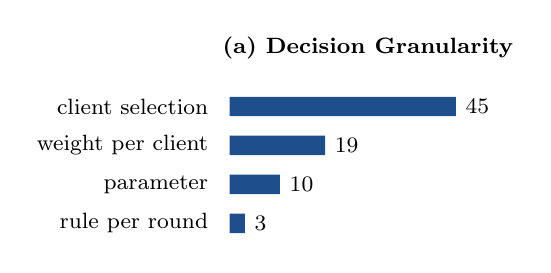
\begin{tikzpicture}
    \begin{axis}[
      eixoh,
      xmax=55,
      title={(a) Decision Granularity},
      symbolic y coords={
        rule per round,
        parameter,
        weight per client,
        client selection
      },
      ytick=data
    ]
      \addplot[fill=barra, draw=none] coordinates {
        (45,client selection)
        (19,weight per client)
        (10,parameter)
        (3,rule per round)
      };
    \end{axis}
  \end{tikzpicture}\hfill
  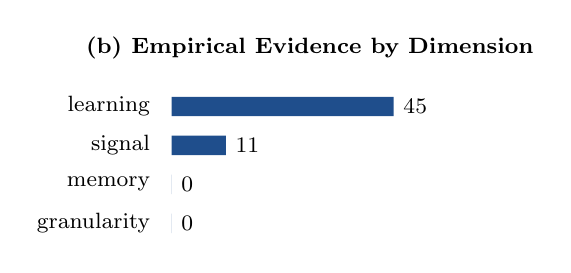
\begin{tikzpicture}
    \begin{axis}[
      eixoh,
      xmax=56,
      title={(b) Empirical Evidence by Dimension},
      symbolic y coords={
        granularity,
        memory,
        signal,
        learning
      },
      ytick=data
    ]
      \addplot[fill=barra, draw=none] coordinates {
        (45,learning)
        (11,signal)
        (0,memory)
        (0,granularity)
      };
    \end{axis}
  \end{tikzpicture}
  \caption{Distribution of studies by decision granularity and experimental isolation of components.}
  \label{fig:eixos}
\end{figure*}
